\section{Autonomous Intersection Management}
\label{sec:aim}

The AIM protocol is based on a \emph{reservation} paradigm, in which
vehicles ``call ahead'' to reserve space-time in the
intersection~\cite{bib:Dresner08Multiagent}. The system assumes that
computer programs called \emph{driver agents} control the vehicles,
while an arbiter agent called an \emph{intersection manager} (IM) is
placed at each intersection.  The driver agents attempt to reserve a
block of space-time in the intersection.  The intersection manager
decides whether to grant or reject requested reservations according to
an \emph{intersection control policy}.  In brief, the paradigm
proceeds as follows.
\begin{small_ind_s_itemize}
\item An approaching vehicle announces its impending arrival to the
IM.  The vehicle indicates its predicted arrival time, velocity,
acceleration, and arrival and departure lanes.
\item The IM simulates the vehicle's path through
the intersection, checking for conflicts with the paths of any
previously processed vehicles.
\item If there are no conflicts, the IM issues a
reservation. It then becomes the vehicle's responsibility to arrive at, and
travel through, the intersection as specified.
\item The car may only enter the intersection once it has successfully
obtained a reservation.
\end{small_ind_s_itemize}
The prototype intersection control policy called \emph{First Come,
First Served} (FCFS) operates by dividing the intersection into a grid
of \emph{reservation tiles}. When a vehicle approaches the
intersection, the intersection manager uses the data in the
reservation request regarding the time and velocity of arrival,
vehicle size, etc. to simulate the intended journey across the
intersection.  At each simulated time step, the policy determines
which reservation tiles will be occupied by the vehicle.  If the
vehicle's space-time request has no conflict, the reservation is
successful; otherwise, the reservation request will be rejected.

Empirical results in simulation demonstrated that the 
reservation system with FCFS can dramatically improve the intersection
efficiency when compared to traditional intersection control
mechanisms~\cite{bib:Dresner08Multiagent}.  Overall, by
allowing for much finer-grained coordination, the simulation-based
reservation system can dramatically reduce per-car delay by two orders
of magnitude in comparison to traffic signals and stop signs.  This
reduction of delays can translate into less traffic
congestion~\cite{bib:Au10Motion,bib:Quinlan10Bringing}, which in turn
leads to better fuel efficiency and lower emissions.

A drawback of FCFS is that it is designed for fully autonomous
vehicles only---it does not work with any vehicles that require human
operations. If any human-driven vehicle appears. Dresner and Stone did
propose a hybrid protocol called FCFS-Signal (a.k.a. FCFS-Light) which
allows human-driven vehicles to share the road with autonomous
vehicles at intersections~\cite{bib:Dresner07Sharing}. However, their
approach has two major drawbacks.  First, the benefits of FCFS-Signal
over conventional traffic signals are relatively small until 90-95\%
of the vehicles on the road are autonomous.  Second, and most
important for this paper, FCFS-Signal cannot take advantage of the
limited autonomous capabilities of semi-autonomous vehicles. There are
useful features that human-driven vehicles could have, that AIM
managers have overlooked. To remedy these issues, this paper
introduces a new autonomous intersection system called \emph{SemiAIM}
that works not only with autonomous vehicles but also with
human-driven vehicles and semi-autonomous vehicles.


\begin{figure}
\centering
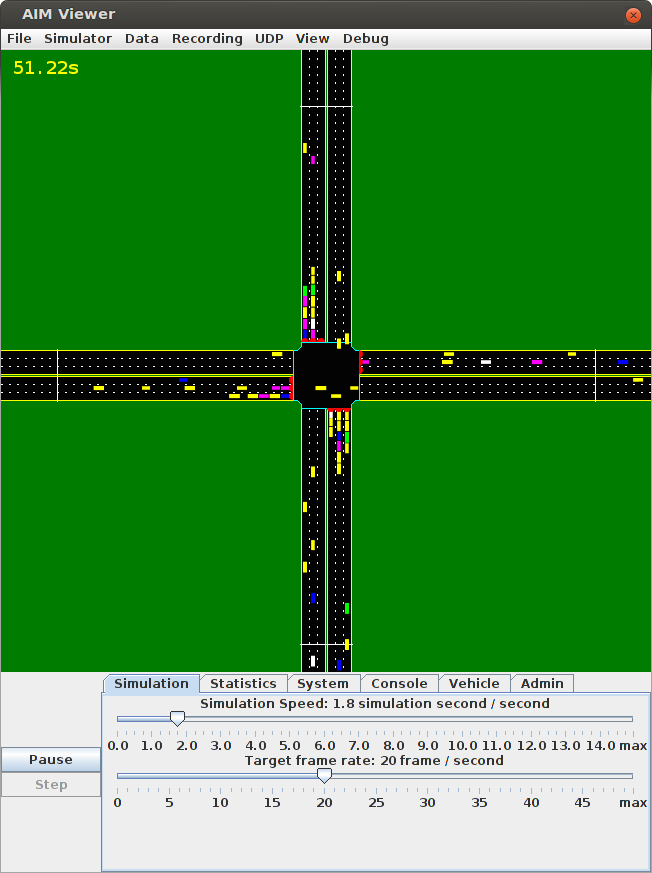
\includegraphics[width=0.8\columnwidth]{figures/demo.png}
\caption{A screenshot of the simulator we developed for the experiments on
SemiAIM.}
\label{fig:simulator}
\end{figure}





% FCFS-Signal (a.k.a. \footnote{It was originally called ``FCFS-Light.''} 


% There are different types of vehicles we'll introduce in
% Section~\ref{sec:vehicles}.


% \commentn {There
% was a paragraph in introduction part describing FCFS-Signal - it was
% called FCFS-light in Dresner's paper. I agree it's better to put it
% here.}



% \commentp{Since we have extra space, there can be a screenshot added
% here.  Also, it would be worthwhile including a description of
% FCFS-signal and describing why that doesn't address the goal of this
% paper (because it assumes that cars are either fully autonomous or
% completely human-controlled).}

%%% Local Variables: 
%%% mode: latex
%%% TeX-master: "gridlock"
%%% End:

